\subsection{广场舞}

中国的广场舞起源于中国群众的生活,是一种由人民集体创造的舞蹈形式。它从中国人民群众中来,又到人民群众中去,是一种即具有娱乐意义,同时又兼顾健身锻炼功能的群众自发创造的艺术文化形式。中国广场舞的主要受众是30到50岁之间的中国妇女群众。这些妇女群众就是大家口中著名的中国大妈。中国大妈们十分热爱这项集体运动。她们十数人,或者数十人乃至上百人,集中在空旷的广场上,伴随着具有摇滚和中国特色的流行音乐,跳着步调和节拍一致的舞蹈。而舞蹈的步调与节拍是由大妈们集体商议而来。而种舞蹈的步调与节拍的灵感有的是来自于专业人士的提议,有的则是由大妈们随心随意而作。大家聚集在广场上跳着广场舞,即不需要表现的有多专业,也没有太多规则的束缚。大妈们想来就来,想走就走,想跳就跳。就算大妈们跳错了也不打紧,跳的不好也没人指责。广场舞突出的就是一个集体娱乐性,集体创造性。这种中国式广场舞的文化起点,就是中国集体的农耕文化。中国人习惯了集体活动,在集体中互相帮助,互相学习,共同创造。农耕文化的记忆深深扎根于广大群众的社会生活之中,使得广场舞成为中国人民喜爱的用以宣泄自身情感,展现民族自信,表达民族文化的一种艺术。
\begin{figure}[htb]
    \centering
  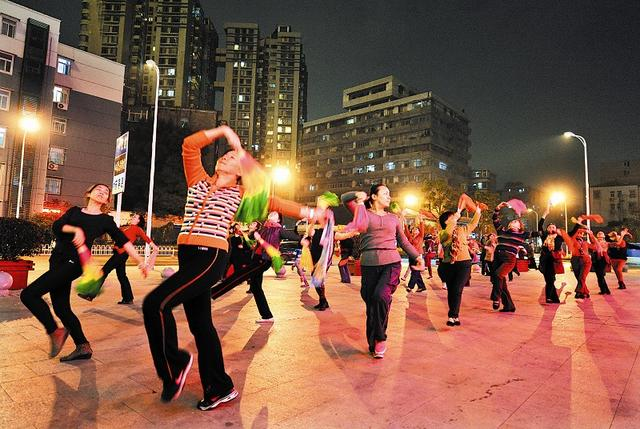
\includegraphics[width=0.6\linewidth]{gcwdm}    
\caption{广场舞大妈}
\end{figure}